\section{SNMP diagnostics and solving problems}
\label{sec:snmp_exports}
This section describes SNMP objects exported by the WR Switch. Objects within
the \texttt{WR\--SWITCH\--MIB} are divided into two groups:
\begin{itemize}
  \item General status objects for operators (section
    \ref{sec:snmp_exports:basic}) - provide a summary about the status of a
    switch and several main subsystems (like timing, networking, OS). These
    should be used by control system operators and users without a
    comprehensive knowledge of the White Rabbit internals. These exports provide
    a general status of the device and high level errors which is enough in most
    cases to perform a quick repair.

  \item Expert objects (section \ref{sec:snmp_exports:expert}) -
    can be used by White Rabbit experts for the in-depth diagnosis of the switch
    failures. These values are verbose and normally should not be used by the
    operators.
\end{itemize}

Description of the general status objects in section
\ref{sec:snmp_exports:basic} includes also a list of actions to follow if a
particular object reports an error. These repair procedures don't require any
in-depth knowledge about White Rabbit. Independently of an error reported, there
are some common remarks that apply to all situations:
\begin{itemize}
  \item Linux inside the WR Switch enumerates WR interfaces starting from 0.
    This means we have to use internally port indexes 0..17. However, the
    port numbers printed on the front panel are 1..18. Syslog messages
    generated from the switch use the Linux port numbering. The consequence is
    that every time Syslog says there is a problem on port X, this refers to
    port index X+1 on the front panel of the switch.
  \item If a procedure given for a specific SNMP object does not solve the
    problem, please contact WR experts to perform a more in-depth analysis of
    the network. For this, you should provide a complete dump of the WRS status
    generated in the first step of each procedure.
  \item The first action in most of the procedures below named \emph{Dump state}
    requires simply calling a tool provided by WR developers that reads all the
    detailed information from the switch and writes it to a single file that can
    be later analyzed by the experts.\\
    {\bf TODO: point to the tool once it's done}
  \item If a problem solving procedure requires restarting or replacing a broken
    WR Switch, please make sure that after the repair, all other WR devices
    connected to the affected switch are synchronized and do not report any
    problems.
  \item If a procedure requires replacing a switch with a new unit, the broken
    one should be handled to WR experts or the switch manufacturer to
    investigate the problem.
\end{itemize}

\subsection{General status objects for operators}
\label{sec:snmp_exports:basic}
This section describes the general status MIB objects that represent the overall
status of a device and its subsystems. They are organized in a tree structure
(fig.\ref{fig:snmp_oper}) where each object reports a problem based on the
status of its child objects. SNMP objects in the third layer of this tree are
calculated based on the SNMP expert objects. Most of the status objects
described in this section can have one of the following values:
\begin{figure}[ht]
  \begin{center}
    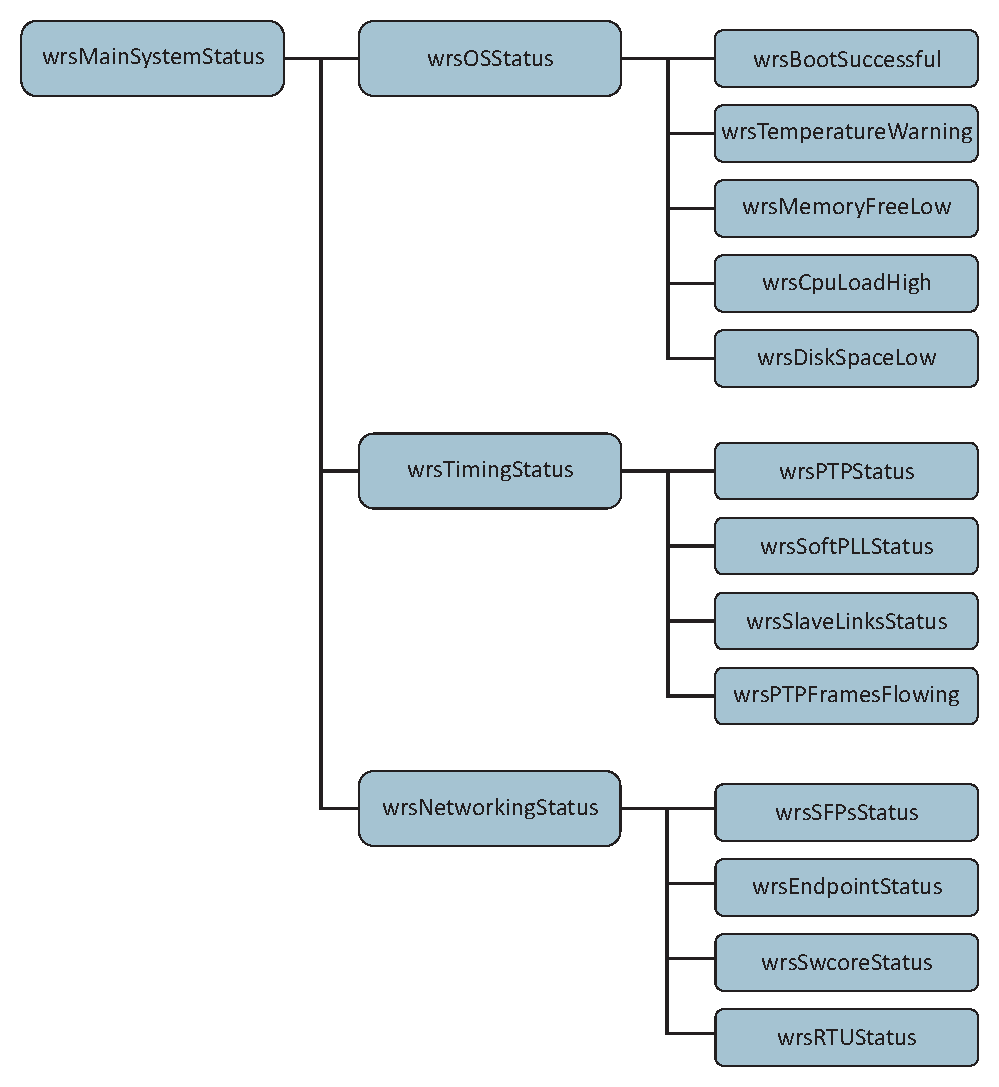
\includegraphics[width=.8\textwidth]{img/snmp_obj.pdf}
    \caption{The structure of general status objects for operators}
    \label{fig:snmp_oper}
  \end{center}
\end{figure}
\begin{itemize}%[leftmargin=0pt]
  \item \texttt{NA} -- status value was not calculated at all (returned value
    is 0). Something bad has happened.
  \item \texttt{OK} -- status of the particular object is correct.
  \item \texttt{Warning} -- objects used to calculate this value are outside the
    proper values, but problem in not critical enough to report \texttt{Error}.
  \item \texttt{WarningNA} -- at least one of the objects used to calculate the
    status has a value \texttt{NA} (or \texttt{WarningNA}).
  \item \texttt{Error} -- error in values used to calculate the particular
    object.
  \item \texttt{FirstRead} -- the value of the object cannot be calculated
    because at least one condition uses deltas between the current and previous
    value. This value should appear only at first SNMP read. To be treated as a
    correct value.
  \item \texttt{Bug} -- Something wrong has happened while calculating the
    object. If you see this please report to WR developers.
\end{itemize}

\paragraph*{SNMP objects:}

% SNMP status objects
\printnoidxglossary[type=snmp_status,title=,style=objtree,sort=def]

\newpage
\subsection{Expert objects}
\label{sec:snmp_exports:expert}

\paragraph*{SNMP objects:}
% SNMP expert objects
\printnoidxglossary[type=snmp_expert,style=objtree,sort=def]

\vspace{12pt}
\paragraph*{Objects from other MIBs:}
% other objects
\printnoidxglossary[type=snmp_other,style=objtree,sort=def]

%%%%%%%%%%%%%%%%%%5
%% Other notes
%
% What else should be reported in the future
% Status of Primary Slave port and backup links
% For backup timing links, report parameters from Backup SPLL channels and PTP servo
% What can be reported regarding eRSTP ?
% %	role of the bridge - root/designated
% % port role - root/designated/backup/alternate/disabled
% % number of exchanged BPDUs
%
% * we could use information from RSTP to visualize the topology of network made of switches
% * switches exchange BPDU messages to leard about other switches
% * RFC 2674 - Bridges with priority, multicast pruning and VLAN
